\documentclass[11pt,a4 paper,title page]{article}
\usepackage[utf8]{inputenc}
\usepackage{natbib}
\usepackage{graphicx}
\usepackage{float}
\usepackage{lineno}
\usepackage[colorlinks = true,
            linkcolor = teal,
            urlcolor  = teal,
            citecolor = black,
            anchorcolor = blue]{hyperref}
  \usepackage{wrapfig}
  \setlength{\pdfpagewidth}{9in} \setlength{\pdfpageheight}{12in}
\usepackage{amsmath}
\usepackage{ragged2e}
\usepackage{hyperref}
\usepackage{epstopdf}

 \title{\textbf{Mini Project :Population Growth}}

\begin{document}
\maketitle
\linenumbers 
 \section{Introduction}
  Malaria is an acute febrile disease. In non-immune individuals, symptoms usually appear 10 to 15 days after being bitten by a mosquito. Plasmodium falciparum malaria can develop into a severe disease, often resulting in death. Anopheles gambiae is the main malaria vector in Africa. Researchers from the Anopheles gambiae 1000 Genome Project sequenced 765 cases of Anopheles gambiae from 15 regions in 8 countries in Africa. Studies have shown that mosquitoes are the most diverse eukaryote, with more than 50 million SNPs identified in accessible genomes \cite{anopheles2017genetic}. These data reveal complex population structures and gene flow patterns, and prove ancient expansion, recent bottlenecks, and local changes in effective population sizes. 
  \hfill\break
  
    In order to commit to malaria control, the "WHO Global Malaria Technical Strategy 2016-2030" adopted by the World Health Assembly in May 2015 provides a technical framework for all malaria-endemic countries \cite{malaria2005world}. It aims to guide and support regional and national plans in efforts to control and eliminate malaria. In addition to chemical methods to control disease vectors, there is also the use of genetic engineering. Genome is the center of malaria research. At present, the genomes of Plasmodium falciparum, the vector mosquito Anopheles gambiae, and humans have all been sequenced. Scientists modify the genes of Anopheles mosquitoes to shorten their lifespan or to fight off malaria \cite{ito2002transgenic}. The study of recombination rate is inseparable from the genetic modification of the human genome.
  \hfill\break
  
  Accurately estimating the complete picture of the recombination rate of the entire genome in a natural population is the main goal of genomics because the way of contact affects everything from genetic maps to understanding evolutionary history \cite{ torada2019imagene}. However, the genetic basis of many complex phenotypes is still largely unknown, mainly due to the environmental factors involved, the polygenicity of traits and the small impact of each associated mutation. Therefore, it is difficult to estimate the characteristics of natural selection in the genome. When only a limited amount of summary statistics is used, these functions are secret, complex, and difficult to detect. To overcome these problems, I explored the application of deep learning in evolutionary biology.
  \hfill\break
  
  Deep learning is a part of machine learning, which is a reasoning framework based on artificial neural network (ANN). ANN consists of input (also called features) and output (response), which are connected by a series of nodes in hidden layers \cite{ agatonovic2000basic}. The input unit receives various forms and structures of information based on an internal weighting system, while the neural network tries to understand the presented information to generate an output report. Just as humans need rules and guidelines to arrive at results or outputs, artificial neural networks also use a set of learning rules (short for backpropagation errors) called backpropagation to refine their output. The artificial neural network will initially go through a training phase, in which it will learn to recognize patterns in the data from visual, auditory or textual aspects. In this monitoring phase, the network compares the output of actual production with the output of expected production. The difference between the two results can be adjusted by backpropagation. This means that the network will run in reverse, from the output unit to the input unit, to adjust its connection weights between the units until the difference between the actual result and the expected result produces the smallest possible error. After training, the ANN can predict the response based on any new data input. Andrew Ng from Coursera said that deep learning is the first class of algorithms. If you feed them more data, performance just keeps getting better \cite{ brownlee2016deep}.
  \hfill\break
  
  However, when using deep learning algorithms, the information needs to be simplified into summary statistics to reduce the data dimension and capture most of the relevant information. For genomic data, an alternative method is to make full use of genomic information and process vertical genomic data through image representation. Each color, called a discrete value, is used to define the appearance of a specific allele. In this way, the detection of markers can be directly transformed into the problem of pattern recognition in image analysis. Under this data representation, Convolutional Neural Network (CNN) is the most suitable algorithm for feature extraction and prediction.
  \hfill\break
  
  CNN is a branch of ANN designed specifically for processing images. Since each pixel will be considered as a unique feature, standard artificial neural networks will become unnecessarily complex. Convolutional neural networks can have tens or hundreds of layers, and each layer learns to detect different features of the image. Apply the filter to each training image at a different resolution and use the output of each convolution image as the input to the next layer. Filters can start with very simple functions (such as brightness and edges) and increase the complexity of the function that uniquely defines the object. CNN uses multiple layers of filtering (called convolution), and each layer processes adjacent pixels grouped in a window and then moves them to cover the entire image \cite{ karpathy2016convolutional}. Then the weights associated with each filter are repeatedly adjusted during the training process to detect information-rich local patterns. Therefore, the convolutional layer also has the additional purpose of automatically extracting information features, and then passing this information as an input unit to several fully connected layers for prediction.
  \hfill\break
  
  In this report, I explored the application of deep learning in evolutionary biology, and implemented a project called ImaGene, which applies convolutional neural networks to population genomic data to detect and quantify natural selection, estimate recombination rates in Anopheles gambiae genomes.
  \hfill\break
  \section{methods and data}

    \subsection{Computing tools}
  In this project, I use three computing tools, python latex and Script. Python is used to filter data from sample data and implement CNN. Script is used to generate simulate data via msms \cite{ ewing2010msms}. Latex is used to write report, make the format more normalization.
  \hfill\break
    \subsection{Data}
  In this project, I use ag10000G as a sample data. Ag1000G samples are sequenced by the Wellcome Trust Sanger Institute Parasites and Microbes Programme(link is external) using Illumina high-throughput technology \cite{ anopheles2014ag1000g}. The sequence data are then used to discover genetic variation between samples and to make genotype calls. Ag1000G is an international collaboration using whole genome deep sequencing to provide a high-resolution view of genetic variation in natural populations of Anopheles gambiae, the principal vector of Plasmodium falciparum malaria in Africa.
  \hfill\break
    \subsection{Methods}
  The propose of this project is use CNN to estimate recombination rates in Anopheles gambiae genomes, I implement it in a user-friendly open source program, ImaGene, available at https://github.com/mfumagalli/ImaGene .
  \hfill\break
  
  Step1: using vcftools get sample data, which is meaningful from ag10000G, read this data from vcf file and store it to Imagene objects.
vcftools is a program designed for working with VCF files, the purpose of vcftools is to provide an easy-to-access method for using complex genetic variation data in the form of VCF files. Because some reason, I cannot download complete data. I just download data of anopheles gambiae from Ghana. After filtering with vcftools, I found that the number of genomes is 67. However, I found that there are many genes in this genetic data that are meaningless, and I need to delete the genotypes whose flag is. And pass. I use --max-missing-count 1 to exclude sites with missing genotypes over all individuals, and use –recode-INFO-all –stdout to get the new vcf file as a sample data for this project. After getting the sample data, read this data and stour it to Imagene objects.
  \hfill\break
  
  Step2: use txt file to store parameters, use script files to call txt file and generate simulation data via msms.
In this step, write a txt file called params to store parameters. This parameters including the path to msms.jar, directory of where I will store the simulation data, reference effective population size, length of the locus in bp, mutation rate in 4*Ne*LEN scale, number of chromosomal copies to simulate as a locus and sample size. For performing a binary or multiclass classification, it need to define these parameters, RHORANGE is range and step for the recombination rate, NREPL is the number of replicates (simulations) per value of recombination rate to be estimated, this data should more then 1000, it will get the better result. Meanwhile, it needs to define NBATCH which is the number of batches for each simulation. For processing msms, it needs to define NTHREADS which is a thread of msms. Generatedataset.sh is a script which can accepts an input file which specifies the parameters of the simulations. Finally use subprocess.call to perform population genomic data simulation, the script divides the simulation into different batches for later training.
  \hfill\break
  
  Step3: run and process simulation data to be used for training the CNN
Before training, please parse the encoded simulation file from msms and convert it into a binary matrix. The method of processing population genomic data is through image representation. The image is a three-dimensional matrix, and the third dimension is color. Since most genetic variations are in dialogue, it is very convenient to convert such full-color images to black and white images. Now reduce the color dimension to length 1, and each pixel encodes the frequency of one of the two alleles in a locus. If the ancestral state of the genome is unknown, recode the alignment so that the allele with the highest frequency in each column is converted to zero, and the allele with the lowest frequency is converted to one. Check the sample allele frequency of the selected allele and choose to impose the middle part of the region. Then, I used different criteria to sort the rows and columns. The data is classified and divided into three categories for subsequent training. In this project, I am divided into 20, 40, 60.
  \hfill\break
  
  Step4: implement, train and evaluate the CNN
In this step, ImaGene interacts directly with Keras \cite{ gulli2017deep} model. ImaGene provides utilities to monitor and evaluate training, and it uses standard methods to perform binary and multi-class classification tasks. Use iteration methods to build the CNN model. In this model, all data needs to be classified and trained in batches. The total number of training samples is 300, but the data of 300*67*205 is very large. In order to reduce the time and memory consumption of the computer when running, select batch training. A batchsize of 32 means that 32 samples are a group.  For this project, I implemented a CNN with two 64-unit and one 128-unit 2D convolutional layers with a kernel size of 3×3 and a stride of 1×1. The convolution layer extracts local features in the picture through the filtering of the convolution kernel. The pooling layer is implemented every time the 2D convolutional layer is completed, and the kernel size is 2×2. A total of three pooling layers have been implemented. The pooling layer can reduce the data dimension more effectively than the convolutional layer. This can not only greatly reduce the amount of calculation, but also effectively avoid overfitting. Finally, a fully connected layer with 64 units is applied to output the result. After each training, I will get the updated score, including the accuracy and loss. When the number of simulations is all completed training, I will get the final generated model. Next, I need to optimize the model, reduce the loss value and increase the value of accuracy by changing the parameters, and plot a confusion matrix. The confusion matrix can more intuitively show the relationship between the predicted value and the true value. If the color is darker, it means the match is higher.
  \hfill\break
  
  Step5: substitute sample data into the CNN model and estimate the recombinate rate
In the end, I used the trained model to estimate the recombination rate of the natural selection category. First, adjust the size of the actual data to match the data used for training. After that, the data is converted into the required format. The model will output a probability vector for the given data, and the sum of this vector is 1
  \hfill\break
  \section{Results}
    \subsection{Image representation of Anopheles gambiae genome data}
  After read sample data from vcf file and store it to Imagene objects, genomic data has been transformed into an image representation. I have one image with 134 rows (equivalent to the number of sampled chromosomal copies) and 2200 columns representing all genomic positions reported.
\begin{figure}[H]
\centering
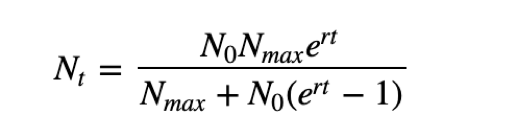
\includegraphics[width=0.9\textwidth,angle=360]{../picture/figure1.png}
\end{figure}
\centerline{Figure 1}

\hfill\break
Figure 1 shows the genome data of anopheles gambiae. it has 134 rows and 1926 columns.  Every row means one chromosome, because anopheles gambiae is diploid, the number of genomes is 67, the number of chromosomes is 134. Every column means genetic locus, it means in this chromosome has 1926 locus. A is the data without sort. The data shown in this picture has no rules to follow, and it is messy. Since the order is arbitrary, no meaning can be seen. So, I can sort rows (and columns) according to several conditions to help feature extraction. B is the data with sort only rows by their distance, arrange from top to bottom according to the distance between the longest appearing lines. C is the data with sort only rows by their frequency, arrange from top to bottom according most frequent haplotypes. With these two sorts, the picture can express the genome more intuitively. On the other hand, each column means a locus and contains information about the relative position of the polymorphism along the locus. The sorting of the columns contains information about linkage disequilibrium, which can provide information for detecting selective sweeps. However, this order is also affected by mutation and recombination events. So, we sort the column. D is the data with sort only columns by their distance, arrange from left to right according to the distance between the longest appearing lines. E is the data with sort only columns by their frequency, arrange from left to right according most frequent haplotypes.
    \subsection{Evaluate pipelines under various data and learning configurations}
  We evaluate whether to change a single parameter to test the choice. In this project, the purpose is to evaluate the accuracy of using CNN to detect and quantify recombination rate events under different learning and data manipulation settings. In this program, 300 pictures can be obtained through msms simulation, each row represents a haplotype randomly sampled from the population. Processing images by sorting rows and columns can improve detection.
\begin{figure}[H]
\centering
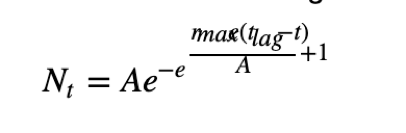
\includegraphics[width=0.25\textwidth,angle=360]{../picture/figure2.png}
\end{figure}
\centerline{Figure 2}
\hfill\break 
Like figure 2, in this project, I implemented a CNN with two 64-unit and a 128-unit 2D convolutional layer with a kernel size of 3×3 and a stride of 1×1. The pooling layer is implemented every time the 2D convolutional layer is completed, and the kernel size is 2×2. A total of three pooling layers have been implemented. Finally, a fully connected layer with 64 units is applied to output the result. At the same time, I deleted the column corresponding to the allele frequency less than 0.015. After sorting, we adjust the size of all images to 67×205 pixels. In order to prevent over-fitting, the "real-time simulation" method is used. The algorithm will train the newly generated data in each cycle. At the same time, it retains the complete training data set. Each cycle separates 10% of the training data for use. As a validation set, 10% of the entire data set is used for testing.
\hfill\break

In order to make my results more convincing, I use the controlled variable method. The controlled variable method is a variance reduction technique used in the Monte Carlo method. It uses the information about the error in the estimation of the known quantity to reduce the error in the estimation of the unknown quantity. This method can eliminate interference and directly reveal the influence of a single factor on the change of the research object. Therefore, in this project, I will make four variable changes to detect and quantify the accuracy of the recombination rate event.
\hfill\break

The initialization parameters are the reference effective population size equals 100000, the length of the locus in bp is 100000, mutation rate in 4*Ne*LEN equals 40, the number of chromosomal copies to simulate equals 100, the range and step for the recombination rate is 20 (in 4N*length units, weak), 40 (medium), 60 (strong). The number of replicates per value of recombination rate to be estimated equals 1000, the number of batches for each simulation equals 10, thread of msms is 4 and every simulation trained on 1-epoch model.
\hfill\break

In the first time, the parameter which is number of batches for each simulation be changed. 10,20,30. In these learning, the total number of images is 600.
\hfill\break 

The number of batches for each simulation equals 10(model 1):
\hfill\break 
The testing results (loss:0.96794 accuracy:0.63833)
\hfill\break 
The value of predict (0.73869,0.24316,0.01815)
\begin{figure}[H]
\centering
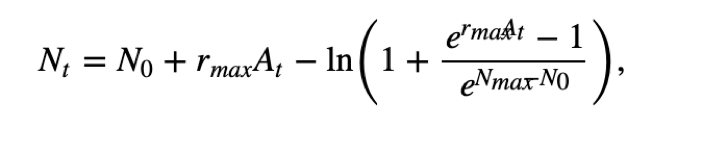
\includegraphics[width=0.5\textwidth,angle=360]{../picture/figure3.png}
\end{figure}
\centerline{Figure 3}
\hfill\break 
\begin{figure}[H]
\centering
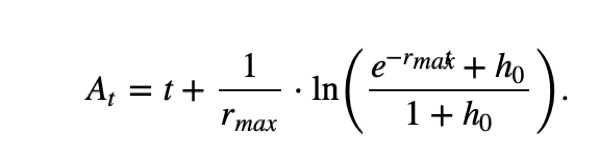
\includegraphics[width=0.5\textwidth,angle=360]{../picture/figure4.png}
\end{figure}
\centerline{Figure 4}
\hfill\break 
Figure 3 shows that the loss value during training and verification in 10 simulations, it shows the value of loss from 15 reduce to 0.9. and Figure 4 shows the confusion matrix. The darkest color means this piece has the highest matching degree. From confusion matrix, I found if choose 20, the accuracy of selection is the highest. When I use this model in the real data, I found the result is as predicted by the model. This means that the model can be used to identify fragments of the genome with a weak recombination rate.
\hfill\break 

The number of batches for each simulation equals 20(model 2):
\hfill\break 
The testing results (loss:0.86217 accuracy:0.66833)
\hfill\break 
The value of predict (0.82825,0.15678,0.01497)
\begin{figure}[H]
\centering
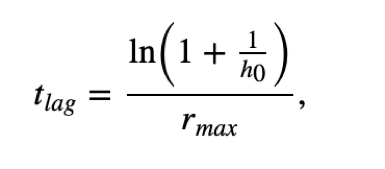
\includegraphics[width=0.5\textwidth,angle=360]{../picture/figure5.png}
\end{figure}
\centerline{Figure 5}
\hfill\break 
\begin{figure}[H]
\centering
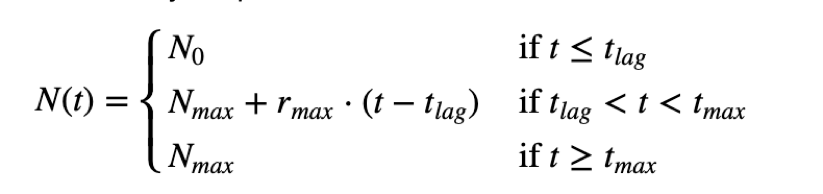
\includegraphics[width=0.5\textwidth,angle=360]{../picture/figure6.png}
\end{figure}
\centerline{Figure 6}
\hfill\break 
Figure 5 shows that the loss value during training and verification in 20 simulations, it shows the value of loss from 15 reduce to 0.86. and Figure 6 shows the confusion matrix. From confusion matrix, I found if choose 20, the accuracy of selection is the highest. When I use this model in the real data, I found the result is as predicted by the model. This means that the model can be used to identify fragments of the genome with a weak recombination rate
\hfill\break 

The number of batches for each simulation equals 30(model 3):
\hfill\break 
The testing results (loss:0.92432 accuracy:0.63833)
\hfill\break 
The value of predict (0.69016,0.27488,0.03496)
\begin{figure}[H]
\centering
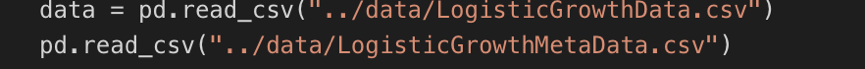
\includegraphics[width=0.5\textwidth,angle=360]{../picture/figure7.png}
\end{figure}
\centerline{Figure 7}
\hfill\break 
\begin{figure}[H]
\centering
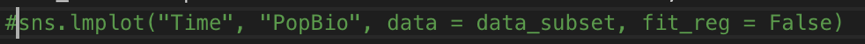
\includegraphics[width=0.5\textwidth,angle=360]{../picture/figure8.png}
\end{figure}
\centerline{Figure 8}
\hfill\break 
Figure 7 shows that the loss value during training and verification in 30 simulations, it shows the value of loss from 15 reduce to 0.92. and Figure 8 shows the confusion matrix. From confusion matrix, I found if choose 60, the accuracy of selection is the highest. When I use this model in the real data, I found that the results are not the same as predicted by the model. This means that the model cannot be used to identify fragments of the genome with a recombination rate
\hfill\break 

Next, the parameter which is the length of the locus in bp is be changed, 100000, 200000, 300000. Cause that, mutation rate in 4*Ne*LEN is be changed, 40, 80, 120.
\hfill\break 

Length of the locus in bp equals 100000, mutation rate in 4*Ne*LEN equals 40(model 4):
\hfill\break 
The testing results (loss:0.96794 accuracy:0.63833)
\hfill\break 
The value of predict (0.73869,0.24316,0.01815)
\hfill\break 
Same as model 1
\hfill\break 

Length of the locus in bp equals 200000, mutation rate in 4*Ne*LEN equals 80(model 5):
\hfill\break 
The testing results (loss:1.15424 accuracy:0.49500)
\hfill\break 
The value of predict (0.83262,0.13596,0.03141)
\begin{figure}[H]
\centering
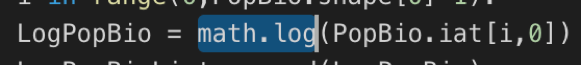
\includegraphics[width=0.5\textwidth,angle=360]{../picture/figure9.png}
\end{figure}
\centerline{Figure 9}
\hfill\break 
\begin{figure}[H]
\centering
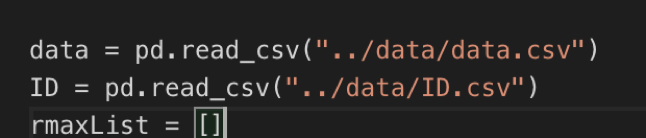
\includegraphics[width=0.5\textwidth,angle=360]{../picture/figure10.png}
\end{figure}
\centerline{Figure 10}
\hfill\break 
Figure 9 shows that the loss value during training and verification when length of the locus in bp equals 200000, mutation rate in 4*Ne*LEN equals 80, it shows the value of loss from 15 reduce to 0.83. and Figure 10 shows the confusion matrix. From confusion matrix, I found if choose 20, the accuracy of selection is the highest. When I use this model in the real data, I found result is as predicted by the model. This means that the model can be used to identify fragments of the genome with a weak recombination rate.
\hfill\break 

Length of the locus in bp equals 300000, mutation rate in 4*Ne*LEN equals 120(model 6):
\hfill\break 
The testing results (loss:1.12191 accuracy:0.51833)
\hfill\break 
The value of predict (0.65387,0.27168,0.07445)
\begin{figure}[H]
\centering
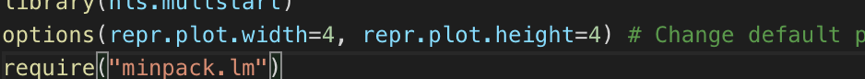
\includegraphics[width=0.5\textwidth,angle=360]{../picture/figure11.png}
\end{figure}
\centerline{Figure 11}
\hfill\break 
\begin{figure}[H]
\centering
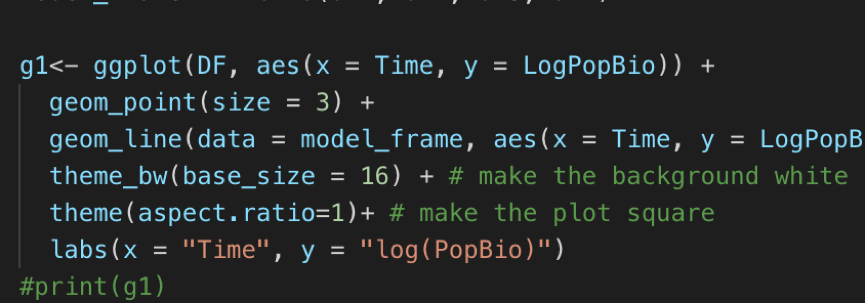
\includegraphics[width=0.5\textwidth,angle=360]{../picture/figure12.png}
\end{figure}
\centerline{Figure 12}
\hfill\break
Figure 11 shows that the loss value during training and verification when length of the locus in bp equals 300000, mutation rate in 4*Ne*LEN equals 120, it shows the value of loss from 15 reduce to 1.12. and Figure 12 shows the confusion matrix. From confusion matrix, I found if choose 20, the accuracy of selection is the highest. When I use this model in the real data, I found result is as predicted by the model. This means that the model can be used to identify fragments of the genome with a weak recombination rate.
\hfill\break

Then, the parameter which is the number of replicates per value of recombination rate to be estimated is be changed. 1000, 3000, 5000.
\hfill\break

The number of replicates per value of recombination rate equals 1000(model 7)
\hfill\break 
Same as model 1
\hfill\break

The number of replicates per value of recombination rate equals 3000(model 8)
\hfill\break 
The testing results (loss:1.12190 accuracy:0.51833)
\hfill\break 
The value of predict (0.65387,0.27168,0.07444)
\begin{figure}[H]
\centering
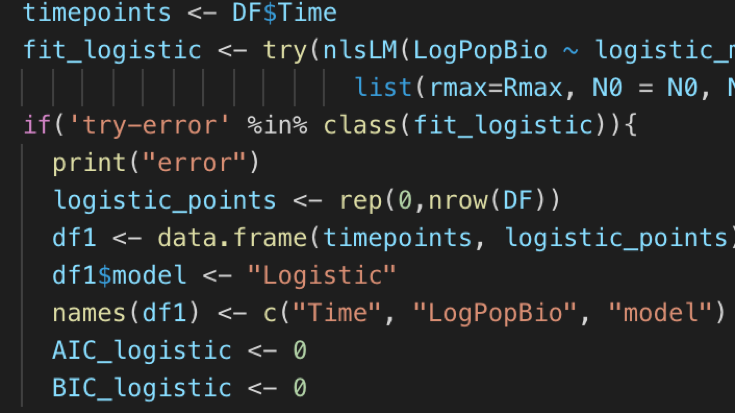
\includegraphics[width=0.5\textwidth,angle=360]{../picture/figure13.png}
\end{figure}
\centerline{Figure 13}
\hfill\break 
\begin{figure}[H]
\centering
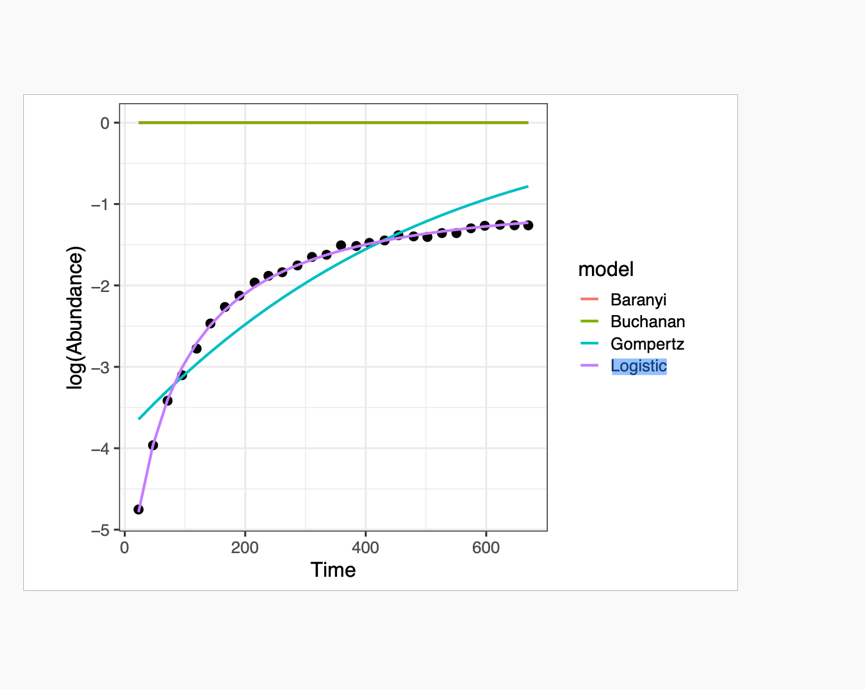
\includegraphics[width=0.5\textwidth,angle=360]{../picture/figure14.png}
\end{figure}
\centerline{Figure 14}
\hfill\break
Figure 13 shows that the loss value during training and verification when the number of replicates per value of recombination rate equals 3000, it shows the value of loss from 15 reduce to 1.12. and Figure 14 shows the confusion matrix. From confusion matrix, I found if choose 20, the accuracy of selection is the highest. When I use this model in the real data, I found result is as predicted by the model. This means that the model can be used to identify fragments of the genome with a weak recombination rate.
\hfill\break

The number of replicates per value of recombination rate equals 5000(model 9)
\hfill\break 
The testing results (loss:0.99253 accuracy:0.63667)
\hfill\break 
The value of predict (0.80850,0.17148,0.02001)
\begin{figure}[H]
\centering
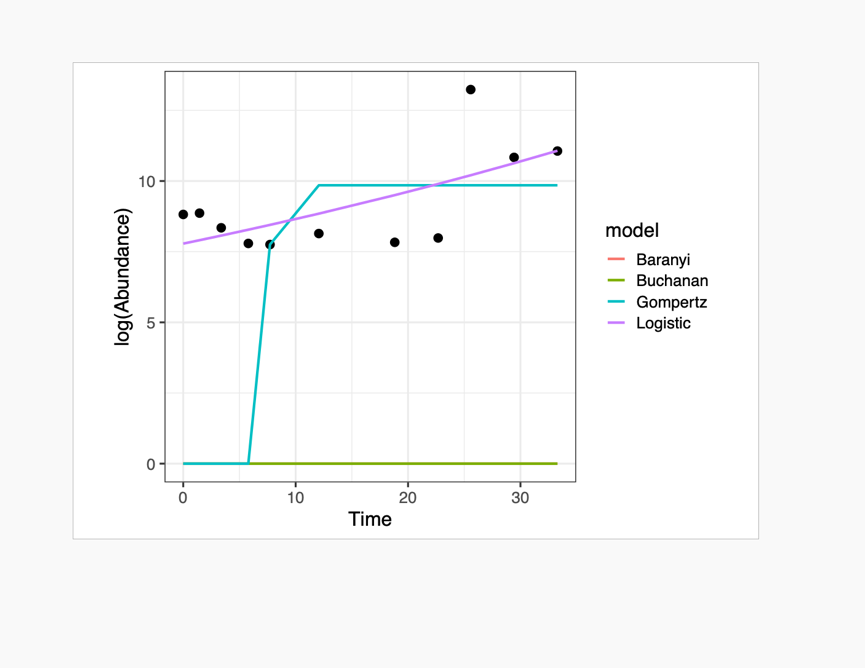
\includegraphics[width=0.5\textwidth,angle=360]{../picture/figure15.png}
\end{figure}
\centerline{Figure 15}
\hfill\break 
\begin{figure}[H]
\centering
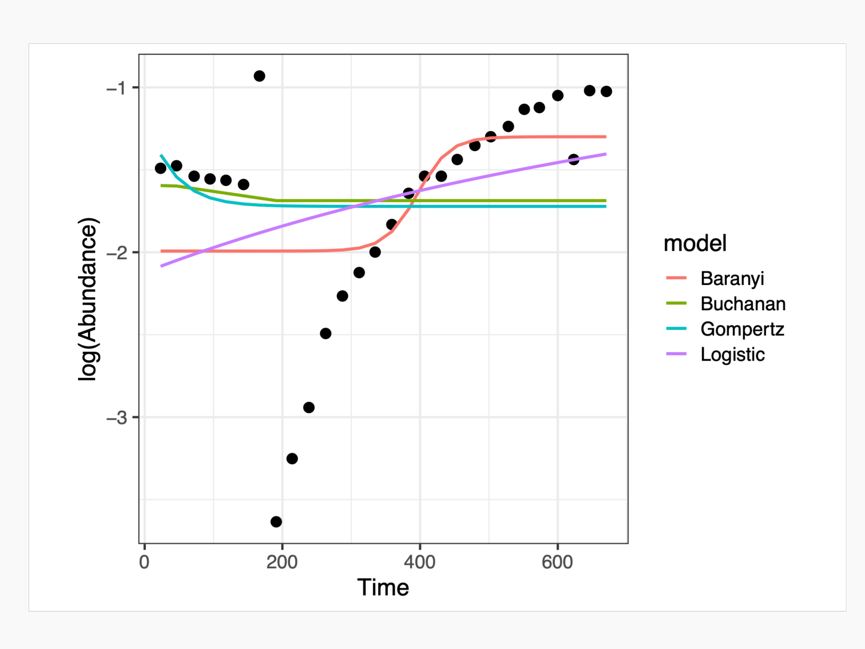
\includegraphics[width=0.5\textwidth,angle=360]{../picture/figure16.png}
\end{figure}
\centerline{Figure 16}
\hfill\break
Figure 15 shows that the loss value during training and verification when the number of replicates per value of recombination rate equals 5000, it shows the value of loss from 15 reduce to 0.99. and Figure 16 shows the confusion matrix. From confusion matrix, I found if choose 60, the accuracy of selection is the highest. When I use this model in the real data, I found that the results are not the same as predicted by the model. This means that the model cannot be used to identify fragments of the genome with a recombination rate.
\hfill\break

Finally, I changed the number of training sessions per simulation. 1-epoch model. 2-epoch model. 3-epoch model.
\hfill\break

every simulation trained on 1-epoch model (model 10):
\hfill\break 
same as model 1
\hfill\break

every simulation trained on 2-epoch model (model 11):
\hfill\break 
The testing results (loss:0.92612 accuracy:0.64667)
\hfill\break 
The value of predict (0.76125,0.21737,0.02139)
\begin{figure}[H]
\centering
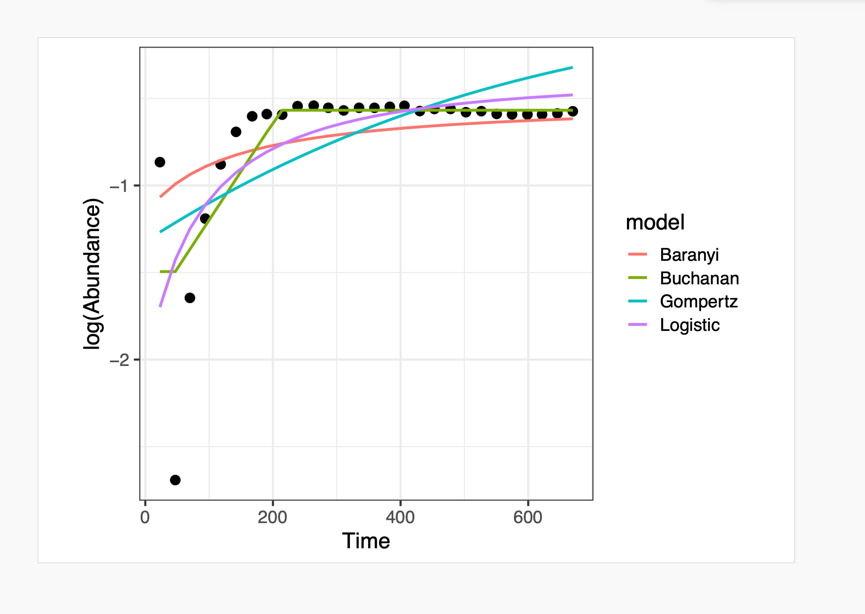
\includegraphics[width=0.5\textwidth,angle=360]{../picture/figure17.png}
\end{figure}
\centerline{Figure 17}
\hfill\break 
\begin{figure}[H]
\centering
\includegraphics[width=0.5\textwidth,angle=360]{../picture/figure18.png}
\end{figure}
\centerline{Figure 18}
\hfill\break
Figure 17 shows that the loss value during training and verification when every simulation trained on 2-epoch model, it shows in the first training, the value of loss from 15 reduce to 0.92. In the second training, the value of loss from 8 to 0.92. Although the initial loss values of the two trainings are different, they will eventually fall to the same loss value. Figure 18 shows the confusion matrix. From confusion matrix, I found if choose 60, the accuracy of selection is the highest. When I use this model in the real data, I found that the results are not the same as predicted by the model. This means that the model cannot be used to identify fragments of the genome with a recombination rate.
\hfill\break

every simulation trained on 3-epoch model (model 12):
\hfill\break 
The testing results (loss:0.85148 accuracy:0.67167)
\hfill\break 
The value of predict (0.73038,0.24809,0.02154)
\begin{figure}[H]
\centering
\includegraphics[width=0.5\textwidth,angle=360]{../picture/figure19.png}
\end{figure}
\centerline{Figure 19}
\hfill\break 
\begin{figure}[H]
\centering
\includegraphics[width=0.5\textwidth,angle=360]{../picture/figure20.png}
\end{figure}
\centerline{Figure 20}
\hfill\break
Figure 19 shows that the loss value during training and verification when every simulation trained on 3-epoch model, it shows in the first training, the value of loss from 15 reduce to 0.85. In the second training, the value of loss from 8 to 0.85. In the last training, the value of loss from 4 to 0.85. Although the initial loss values of the two trainings are different, they will eventually fall to the same loss value. Figure 18 shows the confusion matrix. From confusion matrix, I found if choose 60, the accuracy of selection is the highest. When I use this model in the real data, I found that the results are not the same as predicted by the model. This means that the model cannot be used to identify fragments of the genome with a recombination rate.
\hfill\break  

According to the above model, I think the most model is model 2. Except model 3, model 9, model 11 and model 12, other model can used to identify fragments of the genome with a recombination rate, but if I choose model 2, the value of accuracy is highest.  
\hfill\break  
  \section{Discussion}
In this research, I used ImaGene program, which uses keras to train the CNN model. In this project, I proved that convolutional neural networks have a strong advantage in detecting and quantifying recombination rates of Anopheles gambiae genomes. The use of convolutional neural networks can effectively learn the corresponding features from many samples, avoiding the complex feature extraction process, and more efficiently estimating the gene recombination rate.
\hfill\break  

However, the project still has many parts that need to be improved and expanded to make its predictions more accurate and reliable than the predictions introduced in this article. The random initialization method we choose for setting the initial network parameters before training may not be optimal. Although various tests have been carried out, it is proved that the initial value will optimize the model with modifying the number of simulations. However, the number of tests performed is too few, and more tests are applied to achieve maximum verification accuracy.
\hfill\break  

At the same time, if the units of the convolutional layer are increased, it may have obvious computational advantages. However, further research is needed to evaluate the effect of adjusting the unit size of the convolutional layer, and the trade-off between computational speed and accuracy when increasing the unit size. 
\hfill\break  
Finally, CNN can also be improved, such as using OctConv. OctConv is like the "compressor" of Convolutional Neural Network (CNN) \cite{ chen2019drop}. Using it to replace traditional convolution can improve the effect while saving the consumption of computing resources. For example, for a classic image recognition algorithm, replacing the traditional convolution, the recognition accuracy on ImageNet can be improved by 1.2%, and at the same time, only 82% of the computing power and 91% of the storage space are needed.
\hfill\break  
  \section{Conclusions}
In this research, I used ImaGene, used msms to implement simulation data, and used kares to implement CNN training, detection and quantification of recombination rates. I also learned how data processing and learning settings affect prediction accuracy. 
The discoveries of these efforts will help to change the genes of Anopheles gambiae genomes, better solve the African Malaria, and reveal new associations with complex diseases.
  \bibliographystyle{unsrt}
  \bibliography{ReportBiblio}
\end{document}
